\documentclass[tikz,border=1pt]{standalone}
\usepackage{mathtools}
\begin{document}
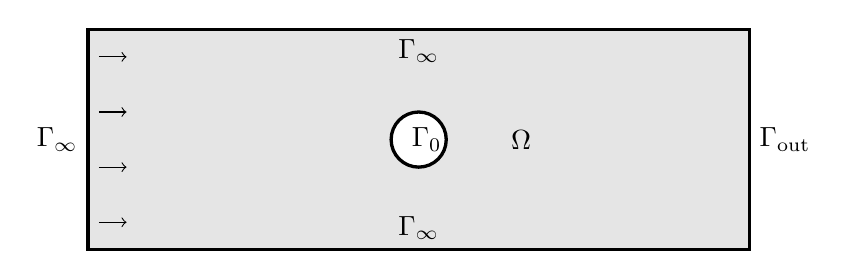
\begin{tikzpicture}[scale=0.7]
\draw[very thick, fill=black!10] (-6, -2) rectangle (6,2);
\coordinate (bl) at (-6,-2);
\coordinate (br) at (+6,-2);
\coordinate (tl) at (-6,+2);
\coordinate (tr) at (+6,+2);
\draw[thick] (bl) --node[above]{$\Gamma_\infty$} (br);
\draw[thick, dashed] (br) --node[right]{$\Gamma_\text{out}$} (tr);
\draw[thick] (tr) --node[below]{$\Gamma_\infty$} (tl);
\draw[thick, dashed] (tl) --node[left]{$\Gamma_\infty$} (bl);
\coordinate (cntr) at (0,0);
\draw[very thick, fill=white] (cntr) circle (0.5);
\node[right] at (-0.3, 0) {$\Gamma_0$};
\node[right] at (1.5, 0) {$\Omega$};
\draw[->] (-5.8, 1.5) -- (-5.3, 1.5);
\draw[->] (-5.8, .5) -- (-5.3, .5);
\draw[->] (-5.8, -.5) -- (-5.3,-.5);
\draw[->] (-5.8, -1.5) -- (-5.3,-1.5);
\end{tikzpicture}
\end{document}
